\documentclass{article}
\usepackage{amsmath}
\usepackage{amssymb}
\usepackage{tikz}
%\usepackage[style=ieee, sorting=ynt, doi=false,isbn=false,url=false,eprint=false, defernumbers=true]{biblatex}
%\addbibresource{papers.bib}

\title{Codec Classifier}
\date{November 17, 2023}

\newcommand{\Rset}{{\cal R}}

\begin{document}

\maketitle

This paper describes a classifier architecture consisting of an encoder and a decoder.  The word ``codec'' in the name Codec Classifier follows from merging the words en{\it co}der and {\it dec}oder.

\begin{figure}
  \begin{center}
  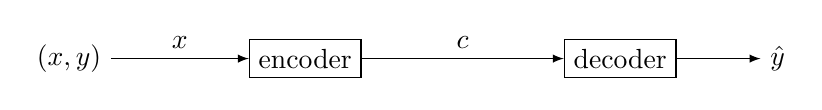
\begin{tikzpicture}[>=latex]
    \node at (-1,0) (x){$(x,y)$};
    \node at (2,0)[draw] (enc){encoder};
    \node at (6,0)[draw] (dec){decoder};
    \node at (8,0) (y){$\hat{y}$};
    \draw[->] (x.east) -- (enc.west) node[above,midway]{$x$};
    \draw[->] (enc.east) -- (dec.west) node[above,midway]{$c$};
    \draw[->] (dec.east) -- (y.west);
  \end{tikzpicture}
\end{center}
\caption{Structure of the codec classifier.}
\label{fig:arch}
\end{figure}

The architecture of the codec classifier is shown in Fig.~\ref{fig:arch}.  An input feature vector $x$ is input to the encoder, which outputs a codeword $c$, which is decoded to a predicted class label $\hat{y}$.  This classifier architecture is reminscent of a communication system.  In communication systems,
\begin{itemize}
  \item the codeword is a perfect representation of the message $x$ with redundancy added to detect and correct errors,
  \item a channel (not shown in Fig.~\ref{fig:arch}) corrupts the bits of the codeword, and
  \item the decoder attempts to recover the message $x$.
\end{itemize}
The decoder's ability to determine $x$ without errors depends on the extent of the channel distortion.

In the classification problem,
\begin{itemize}
\item it is hoped that the codeword $c$ is a perfect representation of the feature vector $x$, but the encoder may be lossy in the sense that $x$ may not be recoverable from $c$,
\item there is no channel, or the channel may be considered to be perfect, i.e. does not induce errors on $c$, and
\item the decoder may be lossy in the sense that even if $x$ is recoverable from $c$, the decoder may not be able to perform that recovery due to the complexity of the recovery problem.
\end{itemize}
In the inferrence step of the classification problem, the goal is to identify the class $y$ associated with an observed $x$.

In communication systems, mutual information is used as a metric to design schemes that make the best use of the channel.  For classification, we adopt the mutual information as a metric to design the encoder and decoder.  We also use the Bayes error as a metric to evaluate different designs.

Consider an encoder consisting of $d$ classification trees having binary codes in the leaves.  A tree with $r$ layers of decision nodes has $2^r$ leaf nodes.  The tree input $x$ selects a leaf node and the leaf's $r$-bit code is output.  Concatenating the results of $d$ trees together yields a $dr$-bit codeword $c$.   A tree with $r=1$ is called a stump.  A stump outputs one bit.  The parameters of a tree are the feature indexes $f_i$, thresholds $t_i$, and $r$-bit codes assigned to the leaves.  The tree output results from a sequence of decisions $x_{f_i} \leq t_i$ that are controlled by the elements of the input feature vector $x$.  When $x_{f_i} \leq t_i$ is true, the decision tree is descended to the left child node and descends to the right child node otherwise.  The classifier design problem chooses the parameters to maximize mutual information or minimize Bayes error.  Under certain conditions, the AdaBoost algorithm is known to minimize the Bayes error.  Therefore, this work builds the encoder with $d$ trees using AdaBoost.

In a multi-class classification problem the AdaBoost classifier may be designed in multiple ways.  Here we offer two possibilities.  First, the standard multi-class AdaBoost approach may be used.  Another possibility is to randomly divide the classes into two sets and train a binary classifier on the sets using the weights from the boosting process.

Suppose the encoder is constructed from $d$ stumps.  Each stump splits feature space into two halfspaces in which the separating hyperplane is aligned with one of the axes.  A stump outputs a 0 for all inputs $x$ in one halfspace and a 1 for all points in the other halfspace.  Put another way, the inverse images of 0 and 1 are axis-aligned halfspaces.

The inverse image of a codeword $c$ is a hyperrectangular set constructed by intersecting one halfspace region from each tree depending on whether the codeword bit is a 0 or a 1.  Codewords and hyperrectangles are in one-to-one correspondence so that we may think of the list of hyperrectangles being indexed by binary codewords.  The hyperrectangles partition feature space into disjoint sets that cover the space.  There are $2^d$ hyperrectangles.  Some of these rectangles may be empty sets.  In that case, the correponding codewords would never be observed at the output of the encoder.

An example classification problem may help to set ideas about the magnitudes of the values involved.  The MNIST dataset consists of $28 \times 28$ 8-bit grayscale images of handwritten digits.  Each image consists of $28^2=784$ pixels.  Each pixel may take on $2^8=256$ values.  Thus there are $(2^8)^{784} = 2^{6272} \approx 10^{1888}$ different images possible.  Suppose we use AdaBoost to build an encoder of $d=1000$ stumps.  There are $2^{1000} \approx 10^{301}$ possible codewords.  Thus, in this case there are not enough codewords to assign a unique codeword to each image.  However, we suppose that feature space may be partitioned into $2^{1000}$ hyperrectangular regions such that a unique codeword can be assigned to each region.  If the regions are pure in the sense that they contain data points from only one class, then the codeword $c$ uniquely represents the class and the decoder design problem is to perform that decoding error free.

An optimal decoder would be an array of $2^d$ elements, i.e. a look-up-table, one element for every hyperrectangle, addressable by the $d$-bit codeword $c$, and storing the class lable $\hat{y}$ for points falling into the corresponding hyperrectangle.  Unfortunately, storing this array exceeds the memory capacity of any conceivable computer for the MNIST dataset and for most other interesting classification problems.  Therefore, we are forced to consider suboptimal approximations of the big look-up-table.

Consider a computer with memory capacity that can store a $2^m$-element array addressed by an $m$-bit word.  This array approximates the $2^d$-element array by sampling $m$ bits out of the $d$ bit codeword $c$.  The particular $m$ bits used may be found by searching over the ${d \choose m}$ combinations of $m$ bits.  However, in interesting classification problems ${d \choose m}$ is so large a number that this search is computationally infeasible.  What is needed is a decoder that approximates the optimal decoder using limited memory and limited computational resources.  We note that heuristic searches such as simulated anealing may find good $m$-bit subcodewords, but we do not pursue this approach further here.

Let $a_{m}$ be an array with $2^m$ elements.  If $w$ is a $m$-bit word, $a_m[w]$ is the corresponding element from array $a_m$.  Let $\sigma_m$ be a selection operator such that $w=\sigma_m(c)$ is an $m$-bit word whos values are selected from codeword $c$.  Composing $\sigma_m$ and $a_m$ gives a definition for a {\it selective array} $a_m[\sigma_m(c)]$, which accesses elements in a small array $a_m$ using select bits $\sigma_m(c)$ from the big codeword $c$.

A tractable, storable approximation to the big look-up-table consists of multiple layers of selective arrays.  Each layer consists of a parallel collection of $d^l$ distinct selective arrays
arrays in which each array is addressed by an $m^l$-bit word.  Each array outputs one bit.  These bits are collected into a $d^l$-bit codeword, which is taken as the input to the selective arrays in the next layer for $l=1, 2, \cdots, L$.  The array in the last layer stores class labels.  The complexity of each layer is determined by the pair $(d^l,m^l)$.  An example network of selective arrays is $(100,5), (50,5), (20,5), (1,20)$.  In this case the last layer has one large array.  The memory requirement is $100 \times 2^5 + 50 \times 2^5 + 20 \times 2^5 + 2^{20} = 5440 + 2^{20} = 1,054,016$ elements.  Most of the memory is for the final array.

The parameters in the proposed decoder are the indexes in the selection operators and the 0/1 bit values stored in the arrays.  We propose a strategy like bagging for finding the selection indexes in $\sigma_m$.  A set of 10 indexes from the input codeword are chosen at random.  Then a ${10 \choose 5}$-way brute force sesarch is performed to select the best 5 from the 10 randomly chosen.  For each five indexes tested, the binary values stored in the array elements are searched at random.  For five bits, there are 32 array elements and $2^{32}$ different combinations possible.  That is too many to exhaustively search.  If instead of 5 bits selected, there were 4, then there would be 16 elements in the array and $2^{16}=65,536$ possible bit configurations.  That might be a small enough number to try all possibilities.  The objective to be maximized during the search is mutual information until the last stage when class labels are output and Bayes error can be minimized, maximizing mutual information between the codeword at the layer output and the input $x$ can be used for optimization.

We note that not all bit patterns need to be tested in the arrays.  For example, an all-zero or all-one array does not help with classification.  Similarly, an array in which the output bit is controlled by one or a few bits in the input word could produce the same output using fewer input bits.  Taking this into consideration only reduces the total number of possiblities by about half, which is not a significant savings.

We propose a greedy approach to optimizing the selective arrays following concepts from building classification trees.  Randomly select a set of bits from the word at the layer input.  Due to the binary nature of the bits, only one splitting point need be considered, $t=0.5$.  Evaluating whether this is a good variable for splitting, calculate the mutual information instead of entropy or Gini index as are commonly used in classification trees.  The mutual information may be evaluated between the class labels $y$ or the data vectors $x$ themselves and the output bits from the split in question.  After selecting a variable for ``splitting'', the dataset is divided and more splits are considered on the next level.  These trees may be grown either sequentially or in parallel.  Note that this architecture leads to a deep network of trees which we call a deep tree network (DTN).

\section{Metrics: Bayes Error}

This section explores Bayes error as a metric for designing coders or decoders for classification.  The Bayes error is the lowest error that can be achieved by any classifier for a classification problem.  Let $f_i = f(x|i)$ be the conditional probability of observing $x$ given that the class is $i$, and let $p_i$ be the priori probability of class $i$.  Then $p_if_i$ is proportional to the posterior probability of $i$ given $x$.  An optimal classifier uses the rule $\hat{i} = \arg\max_i p_i f_i$.  The error associated with this classifer (i.e. the Bayes error) may be computed as
\begin{gather*}
{\cal E} = \int_{p_1 f_1 \leq p_2 f_2} p_1 f_1 dx + \int_{p_1 f_1 \geq p_2 f_2} p_2 f_2 dx. 
\end{gather*}
To simplify the notation, let's define the following shorthand
\begin{gather*}
\int_\leq = \int_{p_1 f_1 \leq p_2 f_2} dx, \qquad \int_\geq = \int_{p_1 f_1 \geq p_2 f_2} dx
\end{gather*}
so that the Bayes error may be written as
\begin{gather*}
{\cal E} = \int_\leq p_1 f_1 + \int_\geq p_2 f_2.
\end{gather*}
Then
\begin{align*}
{\cal E} &= \int_\leq p_1 f_1 + \int_\geq p_2 f_2 \\
&= \frac{1}{2} \left( \int_\leq p_1 f_1 + \int_\geq p_2 f_2 + \int_\leq p_1 f_1 + \int_\geq p_2 f_2 \right) \\
&= \frac{1}{2} \left( \int_\leq p_1 f_1 + \int_\geq p_1 f_1 + \int_\geq p_2 f_2 + \int_\leq p_2f_2 + \int_\leq (p_1 f_1 - p_2f_2) + \int_\geq (- p_1 f_1 + p_2 f_2) \right) \\
&= \frac{1}{2} \left( \int (p_1 f_1 + p_2 f_2) + \int_\leq (p_1 f_1 - p_2f_2) + \int_\geq (- p_1 f_1 + p_2 f_2) \right) \\
&= \frac{1}{2} \left( \int (p_1 f_1 + p_2 f_2) - |p_1 f_1 - p_2f_2| \right) \\
&= \int p_2 f_2 - \int p_2 f_2 + \frac{1}{2} \left( \int (p_1 f_1 + p_2 f_2) - |p_1 f_1 - p_2f_2| \right) \\
&= p_2 + \frac{1}{2} \left( \int (p_1 f_1 - p_2 f_2) - |p_1 f_1 - p_2f_2| \right) \\
&= \min(p_1,p_2) + \max(p_2-p_1,0) - \frac{1}{2} \left( \int f_2 \left[\left(p_2 - p_1 \frac{f_1}{f_2}\right) + \left|p_2 - p_1\frac{f_1}{f_2}\right| \right]\right) \\
&= \min(p_1,p_2) - \int f_2t\left(\frac{f_1}{f_2}\right), \\
&= \min(p_1,p_2) - E_{f_2} t\left(\frac{f_1(X)}{f_2(X)}\right) \\
t(x) &= \frac{1}{2} \left[ (p_2-p_1 x) + |p_2 - p_1 x|\right] - \max(p_2-p_1,0) \\
&= \max(p_2-p_1x,0) - \max(p_2-p_1,0).
\end{align*}

A $f$-divergence between two density functions $f_1$ and $f_2$ is defined as
\begin{gather*}
D_g(f_1 || f_2) = \int f_2(x) g\left(\frac{f_1(x)}{f_2(x)} \right) dx = E_{f_2} \left[g\left(\frac{f_1(X)}{f_2(X)}\right)\right],
\end{gather*}
where $g$ is a smooth and convex function such that $g(1) = 0$.  The KL-divergence, Hellinger distance, and total variation distance are special cases when $g(x) = x \log(x), (1-\sqrt{x})^2, \frac{1}{2} |x-1|$, respectively.  Observe that $t$ satisfies the properties required in the definition of $f$-divergence: $t(1) = 0$ and $t(x)$ is a convex function.  Thus, the expression for the Bayes error above shows it able to be written as an f-divergence between conditional densities $f_1$ and $f_2$.

\subsection{Using Bayes Error with Data}

When observations of $x$ are available under $f_1$ and $f_2$, the ensemble average is replaced by a sample average
\begin{gather*}
\hat{{\cal E}}(X_1,X_2) = \min(\hat{p}_1, \hat{p}_2) - \frac{1}{N_2} \sum_{i=1}^{N_2} \tilde{t}\left(\hat{U}_i\right),
\end{gather*}
where $\tilde(t)(x) = \max(t(x),t(C_L/C_U))$, $0 < C_L \leq f_1(x), f_2(x) \leq C_U$, and $\hat{p}_1,\hat{p}_2$ are emperical estimates (relative frequencies) of the class labels in the training set.  $\hat{U}_i$ is an estimate of the density ratio at point $x_i$ with class label 2, which is computed based on the data points falling into an $\epsilon$-ball about $x_i$, and $N_2$ is the number of class 2 points.

A symmetric version of Bayes error is
\begin{gather*}
{\cal E}_\epsilon = \frac{N_2}{N} \hat{{\cal E}}(X_1,X_2) + \frac{N_1}{N}\hat{{\cal E}}(X_2,X_1) = \min(\hat{p}_1, \hat{p}_2) - \frac{1}{N} \sum_{i=1}^{N} \tilde{t}\left(\hat{U}_i^\epsilon\right),
\end{gather*}
where $\hat{U}_i^\epsilon$ is the density ratio estimate using a $\epsilon$-ball about the point $x_i$ (see Noshad's thesis for the definition).  Estimates for various values of $\epsilon$ may be combined to improve convergence behavior.  See Noshad's thesis for more information.
Noshad's thesis also presents a multi-class version of the Bayes error estimator.

\section{Mutual Information}

\subsection{Nearest Neighbor Ratio (NNR)}

The NNR provides estimates of divergence (either Renyi divergence or $f$-divergence).  The NNR estimate of mutual information is obtained by constructing a second dataset in which the class labels are randomly permuted leading to independence between the features and the labels.  These two datasets are passed into a divergence measure
\begin{gather*}
\hat{I}(X,Y) = \hat{D}((X,PY) || (X,Y)).
\end{gather*}
See chapter 2 in Noshad's thesis for more information on this approach.  A randomized and ensemble version of NNR are also presented with improved performance.  I tend to think that the basic NNR would be sufficient for training/learning the selective arrays by greedy tree building methods.  In this case, we are trying to maximize the mutual information between the input features or their class labels and the binary codes produced in the layers of the trees being built to approximate the selective arrays.  In building a tree that approximates a selective array, splits on various input variables (bits from the codeword produced in the previous layer) are considered.  To evaluate the fitness of any split, pass the training data through the classifier up to the previous layer.  Pass the codeword for each input through the split in question.  This gives a base dataset.  Construct a second dataset in which the class lables are randomly permuted.  Use these two datasets to evaluate a the NNR estimate of mutual information.  One question is whether to use a different random permutation every time or to reuse the same random permutation multiple times when comparing splits on different input variables.  I tend to think that the same permutation should be used when comparing the splits on different input variables because we don't want the randomness in the permutation to bias the variable selection process.  Perhaps several permtuations should be used and the results averaged together to reduce bias.

Maybe this fancy mutual information estimation is unnecessary because our data are discrete and we can simply use histogram estiamtes.  The class labels are few in number and the bits in the binary codes are binary valued.  With a large dataset, the histogram estimates might work very well.

\section{Methodology}

The proposed learning process consists of two steps: (1) learning the encoder that exhaustively segments the input feature space, and (2) learning a decoder that exhaustively labels each region in the segmentation.

\subsection{Encoder: Exhaustive Segmentation}

The first step keeps adding trees or stumps until the feature space is segmented into pure regions or until a desired error rate is achieved.  Pure regions would give zero error on the training set.  The overall classifier will achieve no better error rate than what is enabled by the segmentation.  The tradeoff is that achieving pure regions may require dramatically more regions than achieving a non-zero error rate.  Thus error rate may be used to control the size of the encoder layer.

\subsection{Decoder: Exhaustive Labeling}

An ideal decoder will assign a label to each region created by the encoder.  Because this is usually not possible, a practical decoder, which is subject to memory constraints for storage and to compoutational constraints during learning, is suboptimal.  Finding the optimal is a constrained optimization problem.  Among many options available, we explore the use of bagged or boosted trees to perform a greedy search.

\section{Encoder Training}

In a $k$-class learning problem, two approaches for encoder learning will be explored.  The goal with both approaches is to exhaustively segments (zero error on the training set) or approximately segments (training set error below a predetermined allowable error rate).

\subsection{Approach 1: $k$-class boosting}

The first approach employs the standard multi-class AdaBoost algorithm which augments the objective function with a $k$-dependent term.  The resulting trees contain $k$-element probability vectors in the leaves.  These vectors express the relative frequency of points from the training set that fall into the region corresponding to the leaf.  Pure regions yield one-hot vectors.

\subsection{Approach 2: Randomized Binary Boosting}

The second approach employs a modification to the standard algorithm for binary AdaBoost for learning.  The modification involves two steps.  On each iteration, before the next tree is built, the dataset is divided into two classes rather than $k$-classes.  This is done by a process we call ``splitting the deck''.  As in playing a card game, the class labels are treated as cards, the cards are shuffled to randomize them, and then the deck of cards is randomly split into two sets.  This may be accomplished in code using a random permutation followed by generating a random split point according to some distribution such as a uniform distribution or another distribution such as a binomial distribution that is biased toward splitting the deck in half.  Following this deck-splitting operation, one set of classes is considered the ``0'' class and the other set of classes is considered the ``1'' class.  The next tree is trained to minimize error on this binary segmentation of the dataset.

Why does randomized binary boosting (RBB) properly segment the input feature space?  In simple terms, a classifier that discriminates based on a fine attributes is able to classify based on course attributes.  RBB uses this concept in reverse.  It by learning binary classification on multiple random binary splits of the training data, it learns the finer segmentation.


Let $g$ be a $k$-class classifier $g(x) = i$ if $x \in R_i$ for $i \in I = \{1, 2, \cdots, k\}$, where $R_i$ is the region of the input feature space where the classifier chooses class $i$.  We note that the $R_i$ are disjoint and cover feature space.

Let $h$ be a binary classifier derived from $g$ via a random deck-shuffling operation.  Let $I_a$ and $I_b$ be disjoint index sets corresponding to class $a$ and class $b$ respectively, $I=I_a \cup I_b$.  Let $R_a = \cup_{i \in I_a} R_i$ and $R_b = \cup_{i \in I_b} R_i$ be a disjoint binary partition of the input feature space.  Then $h(x) = a$ if $x \in R_a$ and $h(x) = b$ otherwise.

The error rate of $h$ is
\begin{align*}
{\cal E}_h &= \int_{R_b} p_a f(x|a) dx + \int_{R_a} p_b f(x|b) dx \\
&= \sum_{j \in I_b} \int_{R_j} p_a f(x|a) dx + \sum_{j\in I_a} \int_{R_j} p_b f(x|b) dx \\
&= \sum_{i \in I_a} \sum_{j \in I_b} \int_{R_j} p_i f(x|i) dx + \sum_{i \in I_b} \sum_{j \in I_a} \int_{R_j} p_b f(x|b) dx.
\end{align*}

The error rate of $g$ is
\begin{align*}
{\cal E}_g &= \sum_{i \in I} \sum_{j\neq i} \int_{R_j} p_i f(x|i) dx \\
&= \sum_{i \in I_a} \sum_{j \neq i} \int_{R_j} p_i f(x|i) dx + \sum_{i \in I_b} \sum_{j \neq i} \int_{R_j} p_i f(x|i) dx\\
&= \sum_{i \in I_a} \sum_{j \in I_b} \int_{R_j} p_i f(x|i) dx + \sum_{i \in I_a} \sum_{j \in I_a, j\neq i} \int_{R_j} p_i f(x|i) dx \\
&+ \sum_{i \in I_b} \sum_{j \in I_a} \int_{R_j} p_i f(x|i) dx + \sum_{i \in I_b} \sum_{j \in I_b, j\neq i} \int_{R_j} p_i f(x|i) dx\\
&= {\cal E}_h + {\cal E}_{g,a} + {\cal E}_{g,b}, \\
{\cal E}_{g,a} &= \sum_{i \in I_a} \sum_{j \in I_a, j\neq i} \int_{R_j} p_i f(x|i) dx,\\
{\cal E}_{g,b} &= \sum_{i \in I_b} \sum_{j \in I_b, j\neq i} \int_{R_j} p_i f(x|i) dx,
\end{align*}
where ${\cal E}_{g,a}$ and ${\cal E}_{g,b}$ are the error rates for the $k$-class classifier for particular kinds of errors.  ${\cal E}_{g,a}$ counts errors to classes in the set $I_a$ when $i \in I_a$, and the same for ${\cal E}_{g,b}$.  

Thus we see that the $k$-class error rate is equal to the binary error rate plus the sum of the within class error rates ${\cal E}_{g,a}$ and ${\cal E}_{g,b}$.  However, we note that the error rates derived above are random variables that depend on the distribution of the deck-shuffling operation.  The proposed training process effectively minimizes the binary error rate over multiple draws of deck-shuffling.  Each draw randomizes the membership of classes $a$ and $b$ in the binary problem.  Minimizing the binary error over random draws will minimize the within class error rates.  Thus the $k$-class error rate is minimized in turn.

\section{Related Work}

\subsection{Hashing}

Zhang {\em et al} \cite{fast_knn} describe a method for fast approximate construction of a $k$-nearest neighbor ($k$nn) graph.  They divide a dataset into groups and construct a full $k$nn graph in each group.  The complexity of their method scales with group size.  Division of data into groups is done using hashing in a way that preserves pairwise similarities, i.e. similar items fall into the same group.  This is called locally sensitive hashing (LSH).  In general, a hash has the form
\begin{gather*}
h(x) = [ h_1(x), h_2(x), \cdots, h_m(x) ],
\end{gather*}
where $h_i(x) \in \mathbb{Z}$ (integers).  The specific hash mentioned in the papaer is
\begin{gather*}
h_i(x) = \text{sgn}(w_i^T x + b_i) \in \{-1, +1\},
\end{gather*}
where $w_i$ and $b_i$ are parameters to be learned by an unspecified method.  A datapoint $x$ is placed in a "bucket" by applying the hash map $h(x)$ and then using the $m$-digit $\pm 1$ code as the bucket index.  LSH keeps similar points together using a set of sliced (affine) projections.

The fast $k$nn method uses a binary $\{0,1\}^m$ hash code $y = h(x)$ and uses random projection $w$, $p = w^T y$.  To keep similar points together in groups, the $p$ values are sorted and then blocked into groups of the desired size.  Fully $k$nn graphs are constructed from these groups followed by one stage of neighbor-of-neighbor search.  The whole process is repeated several times using different random projections of the hash codes, and the accuracy of the method is a very good approximation to the full $k$nn graph.

This work is interesting and related for several reasons.
\begin{enumerate}
\item Like this work, we propose to use binary codes.  The binary codes in our method may be thought of as a hash.
\item This method uses learned projections $h_i(x) = \text{sgn}(w_i^T x + b_i)$ to build the has.  Our method uses AdaBoost to construct axis-aligned projections $h_i(x) = \text{sgn}_{\{0,1\}}(e_i^T x - t_i)$ which is equivalent to the logical condition in a decision node $x_i \leq t_i$ in a decision tree.  They do not say how the $w_i$ and $b_i$ are learned in their method.  We follow the principled approach of AdaBoost which has the advantageous claim that it's error approaches the Bayes error (i.e. the best that a classifier can do).
\end{enumerate}

\subsection{Binary and $k$-Class Problems}

Talk in this section about how we propose to handle the $k$-class case either by using multi-class AdaBoost or by using a binary partitioning of the data at each step.  The binary partitioning can be done in multiple ways.  Here we can refer to Singer's one-versus-all splitting or we can follow a random uniform, half-and-half, or $k~$binomial or Poisson splitting.

It may also be a good idea to cover the strong weak learner verses weak weak learner concept here too.

\bibliography{papers.bib}{}
\bibliographystyle{IEEE}
\end{document}
